% !TeX spellcheck = en_US

\documentclass
[
    digital, %% digital / printed
    oneside, %% oneside / twoside
    table, %% table / notable - coloring of tables
    nolof, %% lof / nolof - list of figures inclusion
    nolot, %% lot / nolot - list of tables inclusion
    nocover %% cover / nocover - cover page inclusion
    %% More options at <http://mirrors.ctan.org/macros/latex/contrib/fithesis/guide/mu/fi.pdf>
]{fithesis3}

\usepackage[resetfonts]{cmap}
\usepackage[T1]{fontenc}
\usepackage[main=english, slovak, czech]{babel}

\thesissetup
{
    date = \the\year/\the\month/\the\day,
    university = mu,
    faculty = fi,
    type = mgr,
    author = Bc. Filip Petrovič,
    gender = m,
    advisor = {RNDr. Jiří Filipovič, Ph.D.},
    title = {Framework for Parallel Kernels Autotuning},
    TeXtitle = {Framework for Parallel Kernels Autotuning},
    keywords = {autotuning, parallel programming, OpenCL, CUDA, kernel, optimization},
    TeXkeywords = {autotuning, parallel programming, OpenCL, CUDA, kernel, optimization},
    assignment = {}
}

\thesislong{abstract}
{
    The result of this thesis is a framework for autotuning of parallel kernels which are written in either OpenCL or CUDA language. The framework
    includes advanced functionality such as support for composite kernels and online autotuning. The thesis describes API and internal structure of
    the framework and presents several examples of its utilization for kernel optimization.
}

\thesislong{thanks}
{
    I would like to thank my supervisor Jiří Filipovič for his help and valuable advice, David Střelák and Jana Pazúriková for their feedback and work
    on code examples. I would also like to thank my family for their support during my work on the thesis.
}

%% Insert bibliography
\usepackage{csquotes}
\usepackage
[
    backend=biber,
    style=numeric,
    citestyle=numeric-comp,
    sorting=none,
    sortlocale=auto
    %% More information at <http://mirrors.ctan.org/macros/latex/contrib/biblatex/doc/biblatex.pdf>
]{biblatex}
\addbibresource{references.bib}
\nocite{*}

%% Specify bibliography date format
\DeclareFieldFormat{urldate}
{
    (visited on
    \thefield{urlday}\addslash
    \thefield{urlmonth}\addslash
    \thefield{urlyear}\isdot)
}

%% Index generation
\usepackage{makeidx}
\makeindex

%% Allow extra table formatting commands
\usepackage{array}
\usepackage{ragged2e}
\newcolumntype{L}[1]{>{\RaggedRight\hspace{0pt}}p{#1}}
\newcolumntype{R}[1]{>{\RaggedLeft\hspace{0pt}}p{#1}}

%% Enable inclusion of code samples with coloring
\usepackage{listings}
\usepackage{xcolor}
\definecolor{darkgreen}{rgb}{0.0, 0.6, 0.0}
\definecolor{darkred}{rgb}{0.6, 0.0, 0.0}
\definecolor{lightblue}{rgb}{0.17, 0.57, 0.69}
\definecolor{gray}{rgb}{0.5, 0.5, 0.5}

\lstset
{
    frame=tb,
    language=C++,
    aboveskip=3mm,
    belowskip=3mm,
    showstringspaces=false,
    columns=flexible,
    basicstyle={\footnotesize\ttfamily},
    numbers=none,
    numberstyle=\tiny\color{gray},
    keywordstyle=\color{blue},
    commentstyle=\color{darkgreen},
    stringstyle=\color{darkred},
    breaklines=true,
    breakatwhitespace=true
}

\lstset
{
    emph=[1]{float4, define, elif, endif, def, with, as, in},
    emphstyle=[1]{\color{blue}},
    emph=[2]{size\_t, uint32\_t, PlatformIndex, DeviceIndex, ComputeAPI, KernelId, ArgumentId, string, vector, DimensionVector, unique\_ptr,
        TuningManipulator, ArgumentAccessType, ArgumentMemoryLocation, ModifierType, ModifierAction, ModifierDimension, ParameterPair,
        OutputDescriptor, SearchMethod, function},
    emphstyle=[2]{\color{lightblue}}
}

%% Equations and figures use same numbering
\makeatletter
\let\c@equation\c@figure
\makeatother

%% Make "thanks" section show on top of a page
\makeatletter\thesis@load
\makeatletter
    \def\thesis@blocks@thanks{%
    \ifx\thesis@thanks\undefined\else
    \thesis@blocks@clear
    \begin{alwayssingle}%
    \chapter*{\thesis@@{thanksTitle}}%
    \thesis@thanks
    \end{alwayssingle}%
    \fi}
\makeatother

\begin{document}
\chapter{Introduction}
In recent years, acceleration of complex computations using multi-core processors, graphics cards and other types of accelerators has become
much more common. Currently, there are many devices developed by multiple vendors which differ in hardware architecture, performance and other
attributes. In order to ensure portability of code written for particular device, several software APIs (application programming interfaces) such as
OpenCL (Open Computing Language) or CUDA (Compute Unified Device Architecture) were designed. Code written in these APIs can be run on various
devices while producing the same result. However, there is a problem with portability of performance due to different hardware characteristics of
these devices. For example, code which was optimized for a GPU may run poorly on a regular multi-core processor. The problem may also exist among
devices developed by the same vendor, even if they have comparable parameters and theoretical performance.

A costly solution to this problem is to manually optimize code for each utilized device. This has several significant disadvantages, such as
a necessity to dedicate large amount of resources to write different versions of code and test which one performs best on a given device. Furthermore,
new devices are released frequently and in order to efficiently utilize their capabilities, it is often necessary to rewrite old versions of code and
repeat the optimization process again.

An alternative solution is a technique called autotuning, where program code contains parameters which affect performance depending on their value,
for example a parameter which affects length of a vector type of a particular variable. Optimal values of these parameters might differ for various
devices based on their hardware capabilities. Parametrized code is then launched repeatedly using different combinations of parameters to find out the
best configuration for a particular device.

In order to make autotuning easier to implement in applications, several frameworks were created. However, large number of these are focused
only on a small subset of computations. There are some frameworks which are more general, but their features are limited and usually only support
simple usage scenarios. The aim of this thesis was to develop autotuning framework which would support more complex use cases, such as situations
where computation is split into several smaller programs. Additionally, the framework should be written in a way which would allow its easy
integration into existing software and possibly combine autotuning with regular computation.

The thesis is split into five main chapters. <Todo: add short description of each chapter.>

\chapter{Compute APIs and autotuning}
This chapter serves as an introduction to autotuning technique and includes description of compute APIs which are utilized by KTT (Kernel Tuning
Toolkit)\footnote{Name of autotuning framework developed as a part of the thesis.} -- OpenCL and CUDA. Because both APIs provide relatively similar
functionality, only OpenCL is described here in greater detail. Section about CUDA is mostly focused on explaining features which differ from OpenCL.
It is worth mentioning that CUDA actually consists of two different APIs -- low-level driver API and high-level runtime API built on top of the driver
API. For the purpose of this thesis, only CUDA driver API will be further described, because the runtime API lacks features which are necessary to
implement autotuning in CUDA.

\section{OpenCL}
OpenCL is an API for developing primarily parallel applications which can be run on a range of different devices such as CPUs, GPUs and FPGAs
(field-programmable gate arrays). An OpenCL application consists of two main parts. First part is a host program, which is typically executed on a CPU
and is responsible for OpenCL device configuration, memory management and launching of kernels. Second part is a kernel, which is a function executed
on an OpenCL device and usually contains major part of a computation. Kernels are written in OpenCL C which is based on C programming language.

\subsection{Host program in OpenCL}
Host program is written in a regular programming language, typically in C or C++. Its main objective is to successfully launch a kernel function.
OpenCL API defines several important structures which are referenced from host program:
\begin{itemize}
    \item \textit{cl\_platform} -- References an OpenCL platform.
    \item \textit{cl\_device} -- References an OpenCL device, which is used during context initialization.
    \item \textit{cl\_context} -- Serves as a holder of resources, similar in functionality to an operating system process. Majority of other OpenCL
    structures have to be tied to a specific context. Context is created for one or more OpenCL devices.
    \item \textit{cl\_command\_queue} -- All commands which are executed directly on an OpenCL device have to be submitted inside a command queue. It
    is possible to initialize multiple command queues within a single context in order to overlap independent asynchronous operations.
    \item \textit{cl\_mem} -- Data which is directly accessed by kernel has to be bound to an OpenCL buffer, this includes both scalar and vector
    arguments. It is possible to specify buffer memory location (device or host memory) and access type (read-only, read-write, write-only).
    \item \textit{cl\_program} -- A variable which references OpenCL program compiled from OpenCL C source file. Program can be shared by multiple
    kernel objects.
    \item \textit{cl\_kernel} -- An object used to reference a specific kernel. Holds information about OpenCL program, kernel function name (single
    program can contain definitions of multiple kernel functions) and buffers which are utilized by the kernel.
    \item \textit{cl\_event} -- Serves as a synchronization primitive for individual commands submitted to an OpenCL device. Can be used to retrieve
    information about the corresponding command, such as status or execution duration.
\end{itemize}
Execution of an entire OpenCL application then typically consists of the following steps:
\begin{itemize}
    \item selection of target platform (e.g., AMD, Intel, Nvidia) and device (e.g., Intel Core i5-4690, Nvidia GeForce GTX 970)
    \item initialization of OpenCL context and one or more command queues
    \item initialization of OpenCL buffers (either in host or dedicated device memory)
    \item compilation and execution of kernel function
    \item retrieval of data produced by kernel from OpenCL buffers into host memory (if data is located in dedicated device memory)
\end{itemize}

\subsection{Kernel in OpenCL}
\label{kernel}
Code in a kernel source file is written from perspective of a single \textit{work-item}, which is the smallest OpenCL execution unit. Each work-item
has its own \textit{private memory} (memory which is mapped to e.g., CPU or GPU register).

Work-items are organized into a larger structure called \textit{work-group}, from which they all have access to \textit{local memory} (eg. CPU cache,
GPU shared memory). Work-group is executed on a single \textit{compute unit} (e.g., CPU core, GPU streaming multiprocessor). It is possible for
multiple work-groups to be executed on the same compute unit. OpenCL work-group can have up to three dimensions. Number and size of dimensions affects
work-item indexing inside work-group.

Individual work-groups are organized into \textit{NDRange} (N-Dimensional Range). At NDRange level, it is possible to address two types of memory --
\textit{global memory} and \textit{constant memory}. Global memory (e.g., CPU main memory, GPU global memory) is usually very large but has high
latency. On the other hand, constant memory generally has small capacity but lower latency. It can be utilized to store read-only data. Organization
and indexing of work-groups inside NDRange works in the same way as for work-items inside work-group.

Hierarchical organization into NDRange, work-groups and work-items allows for more intuitive mapping of computation tasks onto OpenCL kernels. Tasks
are defined at the NDRange level, work-groups represent large chunks of a task which are executed in arbitrary order. The smallest operations (e.g.
addition of two numbers) are mapped onto work-items.

Figure \ref{vector_addition} contains a simple OpenCL kernel, which adds up elements from arrays \textit{a} and \textit{b}, then stores the result in
array \textit{c}. Qualifier \textit{\_\_global} specified for the arguments means that they are stored in global memory. Function
\textit{get\_global\_id(int)} is used to retrieve work-item index unique for the entire NDRange in specified dimension.
\begin{figure}
\begin{lstlisting}
__kernel void vectorAddition(__global float* a, __global float* b, __global float* c)
{
    int i = get_global_id(0);
    c[i] = a[i] + b[i];
}
\end{lstlisting}
\caption{Vector addition in OpenCL.}
\label{vector_addition}
\end{figure}

\section{CUDA, comparison with OpenCL}
CUDA is a parallel compute API developed by Nvidia Corporation. It works similarly to OpenCL, but there are also several differences which played an
important role during the framework development:
\begin{itemize}
    \item CUDA is officially supported only on graphics cards released by Nvidia Corporation
    \item Differences in terminology, identical or similar concepts have different terms in OpenCL and CUDA
    \item Global indexing (i.e., NDRange indexing in OpenCL) works differently in CUDA
\end{itemize}
Table \ref{api_terms} contains terms used in OpenCL and their counterparts in CUDA. Due to several differences in design, some terms do not have an
equivalent term in the other API.
\begin{table}[h]
\begin{center}
\begin{tabular}{|*{2}{p{5cm}|}}
    \hline
    OpenCL term & CUDA term \\
    \toprule
    compute unit & streaming multiprocessor \\
    NDRange & grid \\
    work-group & thread block \\
    work-item & thread \\
    global memory & global memory \\
    constant memory & constant memory \\
    local memory & shared memory \\
    private memory & local memory \\
    cl\_platform & N/A \\
    cl\_device\_id & CUdevice \\
    cl\_context & CUcontext \\
    cl\_command\_queue & CUstream \\
    cl\_mem & CUdeviceptr \\
    cl\_program & nvrtcProgram, CUmodule \\
    cl\_kernel & CUfunction \\
    cl\_event & CUevent \\
    \hline
\end{tabular}
\end{center}
\caption{Comparison between OpenCL and CUDA terminology.}
\label{api_terms}
\end{table}

Difference in global indexing plays an important role during addition of tuning parameters which affect either grid dimensions or block dimensions.
In OpenCL, the NDRange size is specified as total number of threads in a dimension. However, in CUDA the grid size is specified as number of threads
in a dimension divided by number of blocks in that dimension. This would be rather inconvenient for porting autotuned programs from one API to the
other. The problem will be further elaborated upon in chapters \ref{ktt-api} and \ref{ktt-structure}.

\section{Possibilities for autotuning in compute APIs}
Design of previously described APIs allows for a wide range of optimization opportunities, both inside kernel and host code. These optimizations can
be implemented with usage of tuning parameters. While some of the parameters can be utilized only in limited range of applications, there are also
several ones which can be implemented in larger number of computation tasks. This section provides a list of some of the most common parameters and
explanation why they are used for autotuning.

\subsection{Work-group (thread block) dimensions}
Work-group dimensions specify how many work-items are included in a single work-group. Work-groups are executed on compute units, which are mapped
onto, for example CPU cores or GPU multiprocessors. Performance of these devices may be vastly different and manually finding an optimal work-group
size is difficult, which is a reason why this parameter usually makes an ideal candidate for autotuning.

\subsection{Usage of vector data types}
Modern processors contain vector registers that allow concurrent execution of a single instruction over multiple data which leads to a significant
speed-up of certain types of computations. Kernel compilers attempt to automatically utilize these registers in order to speed up computation without
manual code modification. However, automatic vectorization is not always optimal. There is an option to perform manual vectorization by using vector
data types which are available in both OpenCL and CUDA. It is possible to control vector length with a tuning parameter, e.g., by using type aliases.

\subsection{Data placement in different types of memory}
Section \ref{kernel} described various memory types available in OpenCL, similar memory hierarchy can also be found in CUDA. In many cases, there are
more valid memory types to choose from for data placement. The choice can have an effect on performance, for example accessing data from OpenCL local
memory is usually faster than using global memory. The problem is that local memory capacity is limited and while on certain devices the data could
fit into it, on other devices it would be necessary to use global memory instead. Having a single version of kernel which would utilize only global
memory would be inefficient for large number of devices. This can be solved by using tuning parameter which controls the data memory placement.

\chapter{Comparison of autotuning frameworks}
This chapter presents several generic autotuning frameworks for parallel kernels. Each section describes one framework, its advantages, disadvantages
and an example of its usage. Frameworks which are not publicly available or focus only on a specific subset of computations are not discussed here.
The final section of this chapter includes motivation for development of KTT framework.

\section{CLTune}
CLTune \cite{cltune} is a framework for autotuning of OpenCL and CUDA kernels. It is freely available in form of a library and provides C++ interface
for writing host programs. It is relatively easy to use and provides capabilities for tuning of single kernels, multiple configuration search
strategies and result validation in a form of reference kernels.

However, it also has several limitations. Among the most significant ones are lack of support for composite kernels, limited argument handling
options and inability to validate kernel results with C or C++ function. The framework is no longer actively developed, so it is unlikely that new
features will be introduced.

Basic tuner configuration in CLTune consists of several main steps, which are listed below. KTT functionality, in its simplest form, is based on the
same idea. Figure \ref{cltune-example} contains part of a program written in CLTune, which includes all the main steps.
\begin{enumerate}
    \item Initialization of tuner by specifying target platform and device.
    \item Addition of tuned kernel.
    \item Addition of reference kernel for output validation.
    \item Definition of tuning parameters.
    \item Setup of kernel arguments.
    \item Launch of the tuning process.
    \item Retrieval of results.
\end{enumerate}
\begin{figure}
\begin{lstlisting}
cltune::Tuner tuner(platformIndex, deviceIndex);
size_t kernelId = tuner.AddKernel({"path/to/kernel.cl"}, "kernelName", ndRangeDimensions, workGroupDimensions);
tuner.SetReference({"path/to/reference_kernel.cl"}, "referenceKernelName", ndRangeDimensions, workGroupDimensions);

tuner.AddParameter(kernelId, "VECTOR_TYPE", { 1, 2, 4, 8 });
tuner.AddParameter(kernelId, "USE_CONSTANT_MEMORY", { 0, 1 });

tuner.AddArgumentInput(bufferA);
tuner.AddArgumentInput(bufferB);
tuner.AddArgumentScalar(helperVariable);
tuner.AddArgumentOutput(bufferResult);

tuner.Tune();
tuner.PrintToScreen();
\end{lstlisting}
\caption{Host program written in CLTune.}
\label{cltune-example}
\end{figure}

In order to support tuning parameters, kernel source file needs to be modified as well. In case of CLTune, the tuner exports parameter values from
given configuration to kernel by using preprocessor definitions. Code needs to be modified, so that the values have intended effect. Simple example
of such modification is shown in figure \ref{cltune-example-kernel}.
\begin{figure}
\begin{lstlisting}
#if USE_CONSTANT_MEMORY == 0
#define MEMORY_TYPE __global
#elif USE_CONSTANT_MEMORY == 1
#define MEMORY_TYPE __constant
#endif

__kernel void tunedKernel(MEMORY_TYPE float* bufferA, ...)
{
    ...
}
\end{lstlisting}
\caption{Adding support for autotuning to kernel via preprocessor macros.}
\label{cltune-example-kernel}
\end{figure}

\section{Kernel Tuner}
Kernel Tuner \cite{kerneltuner} is another open-source kernel autotuning framework. It supports tuning of OpenCL and CUDA kernels as well as regular
C functions, though in the last case, user is responsible for measuring execution duration. API is provided for Python. Compared to CLTune, it
provides more utility methods, for example ability to set kernel compiler options, measuring execution duration in multiple iterations to increase
accuracy and validating output with user-defined, precomputed answer rather than being restricted to reference kernel.

Disadvantages include again lack of support for composite kernels and inability for integration into existing software. However, Kernel Tuner is still
actively developed and some of these shortcomings may be eventually amended.

Host program has to be written in similar fashion as in CLTune, preprocessor definitions for parameters are exported in the same way. Figure
\ref{kerneltuner-example} contains major portion of host program written for Kernel Tuner.
\begin{figure}
\begin{lstlisting}
def tune():

with open('stencil.cl', 'r') as f:
kernel_string = f.read()

problem_size = (4096, 2048)
size = numpy.prod(problem_size)

x_old = numpy.random.randn(size).astype(numpy.float32)
x_new = numpy.copy(x_old)
args = [x_new, x_old]

tune_params = OrderedDict()
tune_params["block_size_x"] = [32*i for i in range(1,9)]
tune_params["block_size_y"] = [2**i for i in range(6)]

grid_div_x = ["block_size_x"]
grid_div_y = ["block_size_y"]

return kernel_tuner.tune_kernel("stencil_kernel", kernel_string, problem_size, args, tune_params, grid_div_x=grid_div_x, grid_div_y=grid_div_y, verbose = True)

if __name__ == "__main__":
    tune()
\end{lstlisting}
\caption{Host program written in Kernel Tuner. Source: \cite{kerneltuner-example}}
\label{kerneltuner-example}
\end{figure}

\section{OpenTuner}
Unlike CLTune and Kernel Tuner, OpenTuner \cite{opentuner} is an autotuning framework which can be used to tune programs written in essentially any
language. API is provided for Python. Due to tuner's more generic nature, users are responsible for writing more sections of code themselves. This
involves, for example writing a method which adds parameter definitions from tuner-generated configurations to tuned program and compiles it. The
other listed frameworks have this functionality already built-in. Another shortcoming is that the framework no longer seems to be actively developed
with majority of the development being done before 2017.

While the other frameworks use preprocessor definitions to export tuning parameters into code, OpenTuner does not have any specific way of parameter
handling. The way parameters become visible in tuned code depends on capabilities of target programming language and on the user-written method for
parameter export. Figure \ref{opentuner-example} contains an example of OpenTuner configuration for tuning of C code. Tuning parameters are added
to code through compiler command line arguments.

\begin{figure}
\begin{lstlisting}
class GccFlagsTuner(MeasurementInterface):

def manipulator(self):
manipulator = ConfigurationManipulator()
manipulator.add_parameter(IntegerParameter('vectorType', 1, 2, 4, 8))
return manipulator

def run(self, desired_result, input, limit):
cfg = desired_result.configuration.data

gcc_cmd = 'g++ tuned_program.cpp '
gcc_cmd += '-VECTOR_TYPE='+ cfg['vectorType']
gcc_cmd += ' -o ./tmp.bin'

compile_result = self.call_program(gcc_cmd)
assert compile_result['returncode'] == 0

run_cmd = './tmp.bin'
run_result = self.call_program(run_cmd)
assert run_result['returncode'] == 0

return Result(time=run_result['time'])

def save_final_config(self, configuration):
print "Optimal vector type written to final_config.json:", configuration.data
self.manipulator().save_to_file(configuration.data, 'final_config.json')
\end{lstlisting}
\caption{Configuration of OpenTuner, source: \cite{opentuner}.}
\label{opentuner-example}
\end{figure}

\section{Development of new framework}
Originally, CLTune was planned to be used as a basis of the new autotuning framework. Extra functionality should simply be added on top of the
existing code structure. However, this has proved to be problematic. While CLTune API is written in a clean and user-friendly manner, its
internal structure made it difficult to extend its functionality. Large part of the internal code is placed into a small number of very long methods
which mix together operations such as argument handling and result validation with accessing compute API functions. This made it difficult to
introduce new features without refactoring large amount of code.

Eventually, it was decided to write a completely new framework, which is called Kernel Tuning Toolkit (KTT). Baseline portion of KTT API remains
similar to CLTune, so it would be easy to port existing programs. However, the internal structure was completely rewritten from scratch, with only
very small portions of CLTune code for following features being reused:
\begin{itemize}
    \item generating of kernel configurations
    \item definition of tuning parameter constraints
    \item configuration searcher based on simulated annealing
\end{itemize}
The new tuner structure is further discussed in chapter \ref{ktt-structure}.

\chapter{KTT API}
\label{ktt-api}
KTT framework API provides users with methods which can be used to develop and tune OpenCL or CUDA applications. It is split into three major
classes, some basic methods were inspired by CLTune. It is available in C++ language.

KTT framework can be acquired from GitHub as a fully open-source library, prebuilt binaries are available for certain platforms. Manual library
compilation is also possible by using build tool premake5, C++14 compiler and CUDA or OpenCL distribution. Supported operating systems include Linux
and Windows.

\section{Tuner class}
Tuner class makes up the main part of KTT API. It includes methods which implement following functionality:
\begin{itemize}
    \item handling of kernels and kernel compositions
    \item handling of kernel arguments
    \item addition of tuning parameters and constraints
    \item kernel running and tuning
    \item kernel output validation
    \item retrieval of tuning results
    \item retrieval of information about available platforms and devices
\end{itemize}

\subsection{Tuner creation}
In order to access the API methods, tuner object has to be created. There are currently three versions of tuner constructors available (figure 
\ref{ktt-constructors}). They allow specification of compute API (either OpenCL or CUDA), platform index, device index and number of utilized compute
queues. OpenCL API with one compute queue is the default setting. Indices are assigned to platforms and devices by KTT framework, they can be retrieved
with a method.

\begin{figure}
\begin{lstlisting}
Tuner(const PlatformIndex, const DeviceIndex)
Tuner(const PlatformIndex, const DeviceIndex, const ComputeAPI)
Tuner(const PlatformIndex, const DeviceIndex, const ComputeAPI, const uint32_t computeQueueCount)
\end{lstlisting}
\caption{Tuner constructors.}
\label{ktt-constructors}
\end{figure}

\subsection{Kernel handling}
Kernels can be added to tuner from a file or C++ string (figure \ref{ktt-kernel-methods}). Users furthermore need to specify kernel function name and
default global and local sizes (i.e., dimensions for NDRange / grid and work-group / thread block). The sizes are stored inside \textit{DimensionVector}
objects, which are a part of KTT framework. They allow easy thread size manipulation and support up to three dimensions. Existing kernels can be
referenced by using a handle returned by tuner. Kernel compositions can be added by specifying handles of kernels included inside composition. In
order to use compositions, user additionally has to define a tuning manipulator class, whose usage is detailed in subsection <todo: add reference>.
\begin{figure}
\begin{lstlisting}
KernelId addKernel(const std::string& source, const std::string& kernelName, const DimensionVector& globalSize, const DimensionVector& localSize)
KernelId addKernelFromFile(const std::string& filePath, const std::string& kernelName, const DimensionVector& globalSize, const DimensionVector& localSize)
KernelId addComposition(const std::string& compositionName, const std::vector<KernelId>& kernelIds, std::unique_ptr<TuningManipulator>)
\end{lstlisting}
\caption{Kernel addition methods.}
\label{ktt-kernel-methods}
\end{figure}
\subsection{Kernel argument handling}
There are three types of kernel arguments supported by KTT -- vector, scalar and local memory (OpenCL) arguments (figure \ref{ktt-argument-methods}).
All arguments are referenced by using a handle provided by tuner. Argument addition methods are templated and support primitive data types (e.g.,
int, float) as well as user-defined data types (e.g., struct, class). Arguments are bound to kernels by using a method which accepts kernel handle
and corresponding argument handles. This allows them to be shared among multiple kernels.

Vector arguments are added from C++ vector containers. It is possible to specify access type (read, write or combined), memory location from where
argument data is accessed by kernel (device or host) and whether argument copy should be made by tuner. By default, copies of all vector arguments
are made by tuner, so the original vectors remain modifiable by user without interfering with tuning process. In case argument is placed in host
memory, it is possible to utilize zero-copy feature, which means that kernel has direct access to buffer which was initialized from host code. This
functionality is supported by both CUDA and OpenCL. All of the vector argument handling options are illustrated with diagram \ref{ktt-buffer-diagram}.

\begin{figure}
\begin{lstlisting}
ArgumentId addArgumentVector(const std::vector<T>& data, const ArgumentAccessType)
ArgumentId addArgumentVector(std::vector<T>& data, const ArgumentAccessType, const ArgumentMemoryLocation, const bool copyData)
ArgumentId addArgumentScalar(const T& data)
ArgumentId addArgumentLocal(const size_t localMemoryElementsCount)
void setKernelArguments(const KernelId, const std::vector<ArgumentId>&)
\end{lstlisting}
\caption{Argument handling methods.}
\label{ktt-argument-methods}
\end{figure}

\begin{figure}
\begin{center}
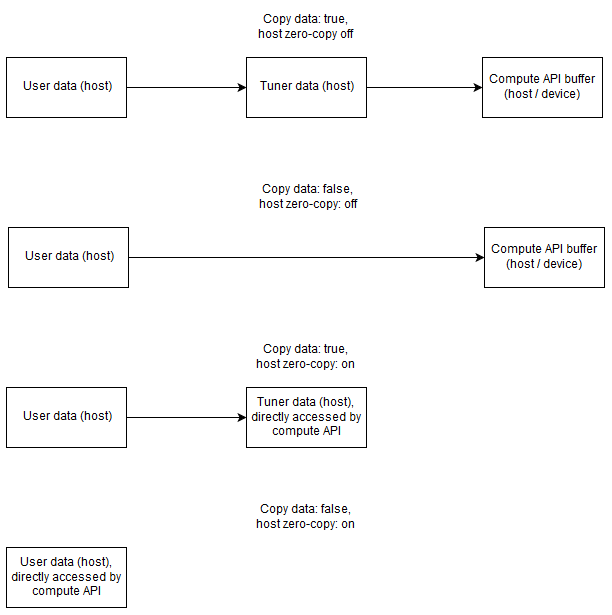
\includegraphics[width=125mm]{resources/ktt_buffer_diagram.png}
\end{center}
\caption{Vector argument handling options in KTT framework. Each box represents one copy of a buffer.}
\label{ktt-buffer-diagram}
\end{figure}

\subsection{Tuning parameters and constraints}
Tuning parameters are specified for kernels with a name and list of valid values. Both integer and floating-point values are supported. Before kernel
tuning begins, configurations for each combination of kernel parameter values are generated. For example, adding parameter A with values 1 and 2, and
parameter B with values 5 and 10 will result in four configurations being generated -- {A1, B5}, {A1, B10}, {A2, B5} and {A2, B10}. Tuned kernel is
then launched with parameter definitions prepended to kernel source code based on the current configuration.

Some tuning parameters may additionally affect global and local sizes of tuned kernel. This is useful, for example in cases where parameter in kernel
source code modifies amount of work done by a single work-item and therefore changes total number of needed work-items. Each dimension can be modified
separately, supported modifiers include addition, subtraction, multiplication and division.

If certain combination of tuning parameters are invalid or unsupported by kernel source code, they can be eliminated by using parameter constraints.
Constraint is a function which accepts list of parameter values for specified parameters and returns a boolean value which signifies whether the values
are valid or not. Constraint conditions are defined by user.

Tuning parameters for kernel compositions are added separately and are independent from kernels. Individual kernels are not affected by composition
parameters either.

\begin{figure}
\begin{lstlisting}
void addParameter(const KernelId, const std::string& parameterName, const std::vector<size_t>& parameterValues)
void addParameterDouble(const KernelId, const std::string& parameterName, const std::vector<double>& parameterValues)
void addParameter(const KernelId, const std::string& parameterName, const std::vector<size_t>& parameterValues, const ModifierType, const ModifierAction, const ModifierDimension)
void addConstraint(const KernelId, const std::function<bool(std::vector<size_t>)>& constraintFunction, const std::vector<std::string>& parameterNames)
\end{lstlisting}
\caption{Tuning parameter and constraint addition methods.}
\label{ktt-parameter-methods}
\end{figure}

\subsection{Kernel tuning and running}
KTT supports offline and online kernel tuning as well as regular kernel running. In offline tuning, kernel configurations are tested iteratively one
after another without interruption. This mode is strictly focused on finding the best performing configuration, retrieval of kernel output by user and
swapping of kernel argument data between configurations is not possible. On the other hand, it allows efficient validation of output. Because the
argument data remains the same for all configurations, the reference output needs to be computed only once.

In online tuning, single configuration is tested at time, enabling combination with kernel running. It also allows kernel output retrieval with
KTT built-in structure \textit{OutputDescriptor}. This structure specifies handle of argument to be retrieved, output memory location and optionally
size of the retrieved data, which is useful in case only part of the argument is needed. Online tuning also enables swapping of argument data between
each configuration, though if validation is enabled, reference output needs to be recomputed every time new configuration is run.

In both modes, the order and number of tested configurations depends on utilized search method. KTT currently supports four search methods -- full
search, random search, simulated annealing and Markov chain Monte Carlo. Full search simply explores all configurations iteratively. The other three
methods allow specification of a fraction parameter which controls number of explored configurations (e.g., setting fraction to 0.5 will result in
50\% of all configurations being tested). In random search, the explored configurations are chosen randomly, while the last two methods employ
probabilistic techniques in order to find configurations with good performance more quickly.

Kernel running supports output retrieval in same fashion as online tuning. However, the configuration to run kernel with is specified by user. Validation
is not performed during kernel running.

\begin{figure}
\begin{lstlisting}
void tuneKernel(const KernelId)
void tuneKernelByStep(const KernelId, const std::vector<OutputDescriptor>& output)
void runKernel(const KernelId, const std::vector<ParameterPair>& configuration, const std::vector<OutputDescriptor>& output)
void setSearchMethod(const SearchMethod, const std::vector<double>& arguments)
\end{lstlisting}
\caption{Kernel tuning and running methods.}
\label{ktt-tuning-methods}
\end{figure}

\subsection{Output validation}
Todo...

\section{Reference class}
Todo...

\section{Tuning Manipulator class}
Todo...

\chapter{KTT Structure}
\label{ktt-structure}
Todo...

\chapter{Conclusion}
Todo...

%% Print full bibliography, use biber.exe on .bcf file to generate bibliography
\csname captions\languagename\endcsname
\makeatletter
\thesis@selectLocale{\thesis@locale}\makeatother
\printbibliography[heading=bibintoc]

\appendix
\chapter{Appendix}
Todo...

\end{document}
